% !TeX program = xelatex
% !TeX TS-program = xelatex
\documentclass[11pt,a4paper,oneside,openany]{book}

% Professional book infrastructure (Phase 7 polish).
% Phase 8 adds final TikZ diagrams, Python graphs, tables, and polished content.

% --- Layout ---
\usepackage[
  a4paper,
  top=2.8cm,
  bottom=2.8cm,
  inner=3.0cm,
  outer=2.2cm,
  headheight=14pt,
  footskip=28pt,
]{geometry}

\usepackage{graphicx}
\usepackage{xcolor}
\usepackage{amsmath}
\usepackage{booktabs}
\usepackage{tabularx}
\usepackage{longtable}

% --- Professional color palette ---
\definecolor{titleNavy}{RGB}{18,52,94}
\definecolor{titleBlue}{RGB}{32,82,130}
\definecolor{boxBg}{RGB}{236,242,249}
\definecolor{boxFrame}{RGB}{176,198,222}
\definecolor{accentOrange}{RGB}{214,96,44}
\definecolor{insightAccent}{RGB}{46,125,90}
\definecolor{warningAccent}{RGB}{180,55,40}
\definecolor{mutedText}{RGB}{90,98,110}

% --- LuaLaTeX / XeLaTeX fonts and Hebrew--English BiDi ---
\usepackage{fontspec}
\usepackage{polyglossia}
\setmainlanguage{english}
\setotherlanguage{hebrew}
\IfFontExistsTF{Segoe UI}{
  \setmainfont{Segoe UI}
  \newfontfamily\hebrewfont[Script=Hebrew]{Segoe UI}
}{
  \setmainfont{Latin Modern Roman}
  \newfontfamily\hebrewfont[Script=Hebrew]{Arial}
}

\usepackage{csquotes}

% --- Styled chapter and section headings ---
\usepackage{titlesec}
\titleformat{\chapter}[display]
  {\normalfont\huge\bfseries\color{titleNavy}}
  {\chaptertitlename\ \thechapter}
  {12pt}
  {\Huge}
\titlespacing*{\chapter}{0pt}{-10pt}{24pt}

\titleformat{\section}
  {\normalfont\Large\bfseries\color{titleBlue}}
  {\thesection}
  {0.8em}
  {}

\titleformat{\subsection}
  {\normalfont\large\bfseries\color{titleNavy}}
  {\thesubsection}
  {0.8em}
  {}

% hyperref after most packages; before fancyhdr per convention
\usepackage[colorlinks=true,linkcolor=titleBlue,urlcolor=titleBlue,citecolor=insightAccent]{hyperref}
\usepackage{fancyhdr}

% --- TikZ (Phase 8 diagrams) ---
\usepackage{tikz}
\usetikzlibrary{arrows.meta,positioning,fit,backgrounds}

% --- tcolorbox infrastructure for Phase 8 content ---
\usepackage{tcolorbox}
\tcbuselibrary{skins,breakable}

\tcbset{
  bookbox/.style={
    enhanced,
    breakable,
    colback=boxBg,
    colframe=boxFrame,
    boxrule=0.6pt,
    arc=3pt,
    left=8pt,
    right=8pt,
    top=6pt,
    bottom=6pt,
    fonttitle=\bfseries,
  },
}

\newtcolorbox{insightbox}[1]{%
  bookbox,
  title={#1},
  colframe=insightAccent,
  colback=boxBg,
  coltitle=insightAccent,
}

\newtcolorbox{warningbox}[1]{%
  bookbox,
  title={#1},
  colframe=warningAccent,
  colback=boxBg!80!white,
  coltitle=warningAccent,
}

\newtcolorbox{formulabox}[1]{%
  bookbox,
  title={#1},
  colframe=titleBlue,
  colback=white,
  coltitle=titleBlue,
}

\newtcolorbox{chapterintrobox}{%
  bookbox,
  title={Chapter Overview},
  colframe=titleNavy,
  coltitle=titleNavy,
}

\newcommand{\chapterbanner}[1]{%
  \par\noindent
  \colorbox{titleNavy}{%
    \parbox{\dimexpr\linewidth-2\fboxsep}{%
      \vspace{4pt}%
      {\color{white}\bfseries\large #1}%
      \vspace{4pt}%
    }%
  }%
  \par\vspace{12pt}%
}

% --- Bibliography ---
\usepackage[backend=biber,style=authoryear,sorting=nyt]{biblatex}
\addbibresource{references.bib}

% --- Headers and footers ---
\pagestyle{fancy}
\fancyhf{}
\fancyhead[LE,RO]{\nouppercase{\color{mutedText}\leftmark}}
\fancyhead[LO,RE]{\color{mutedText}\booktitle}
\fancyfoot[C]{\color{mutedText}\thepage}
\renewcommand{\headrulewidth}{0.4pt}
\renewcommand{\footrulewidth}{0pt}
\renewcommand{\headrule}{\hbox to\headwidth{\color{boxFrame}\leaders\hrule height \headrulewidth\hfill}}

\fancypagestyle{plain}{%
  \fancyhf{}%
  \fancyfoot[C]{\color{mutedText}\thepage}%
  \renewcommand{\headrulewidth}{0pt}%
  \renewcommand{\footrulewidth}{0pt}%
}

\newcommand{\booktitle}{AI Agents That Replace Real Work}
\newcommand{\booksubtitle}{The Future of Automation}


\begin{document}

% --- Formal academic cover page ---
\begin{titlepage}
  \thispagestyle{empty}
  \begin{tikzpicture}[remember picture,overlay]
    \fill[titleNavy] (current page.north west) rectangle ([yshift=-2.6cm]current page.north east);
    \fill[boxBg] ([yshift=7.2cm]current page.south west) rectangle (current page.south east);
    \draw[titleBlue, line width=0.9pt]
      ([xshift=2.2cm,yshift=-2.0cm]current page.north west) --
      ([xshift=6.5cm,yshift=-2.0cm]current page.north west);
    \foreach \x/\y in {4.0/-1.1, 5.8/-1.6, 7.6/-1.2, 9.4/-1.7} {
      \fill[white, opacity=0.2] ([xshift=\x cm, yshift=\y cm]current page.north west) circle (0.07cm);
    }
    \draw[white, opacity=0.16, line width=0.5pt]
      ([xshift=4.0cm,yshift=-1.1cm]current page.north west) --
      ([xshift=5.8cm,yshift=-1.6cm]current page.north west) --
      ([xshift=7.6cm,yshift=-1.2cm]current page.north west) --
      ([xshift=9.4cm,yshift=-1.7cm]current page.north west);
  \end{tikzpicture}

  \vspace*{3.0cm}
  {\Huge\bfseries\color{titleNavy}\booktitle\par}
  \vspace{0.45cm}
  {\Large\bfseries\color{titleBlue}\booksubtitle\par}

  \vspace{1.8cm}
  \begin{center}
    \begin{tikzpicture}
      \draw[titleBlue, opacity=0.45, line width=0.7pt] (0,0) circle (0.55cm);
      \draw[titleNavy, opacity=0.35, line width=0.7pt] (1.1,0.15) circle (0.35cm);
      \draw[titleBlue, opacity=0.3, line width=0.6pt] (-0.9,0.2) circle (0.28cm);
      \draw[boxFrame, line width=0.6pt] (0,0) -- (1.1,0.15);
      \draw[boxFrame, line width=0.6pt] (0,0) -- (-0.9,0.2);
    \end{tikzpicture}
  \end{center}

  \vspace{2.0cm}
  \begin{center}
    \fcolorbox{boxFrame}{boxBg}{%
      \begin{minipage}{0.62\textwidth}
        \vspace{0.55em}
        \renewcommand{\arraystretch}{1.55}
        \begin{tabular}{@{}>{\bfseries}l@{\hspace{1.4em}}l@{}}
          Authors: & Eman Sarhan, Amir Fadila \\[0.35em]
          Course: & Orchestration of AI Agents \\[0.35em]
          Lecturer: & Dr. Yoram Segal \\[0.35em]
          Date: & June 8, 2026 \\
        \end{tabular}
        \vspace{0.55em}
      \end{minipage}%
    }
  \end{center}
  \vspace{1.6cm}
\end{titlepage}

\pagenumbering{roman}
\pagestyle{plain}
\tableofcontents
\clearpage

\pagenumbering{arabic}
\mainmatter
\pagestyle{fancy}

% --- Chapter 1: research-based introduction ---
\chapter{AI Agents and Real Work}
\begin{chapterintrobox}
Tool-enabled AI agents are entering operational workflows that once depended entirely on
human coordination. This chapter introduces what agents are, how they differ from chatbots,
and why task-level automation---with human oversight---is the credible frame for the future
of work \cite{mediumworkflowagents}.
\end{chapterintrobox}
\IfFileExists{.build/generated/chapter_01.tex}{%
  ```latex
\section{Introduction: When AI Agents Start Doing Real Work}

The integration of AI agents into various domains raises critical questions regarding their capabilities and limitations. This discussion focuses on the transformative potential of AI agents, particularly the role of DeepAgent, which is recognized for its advancements in workflow automation.

It is essential to acknowledge the current state of AI agents as they pertain to the workforce. While research suggests that AI agents could significantly alter workflows, it is important to frame these changes as possibilities rather than certainties. For instance, the assertion that \textit{AI agents are set to revolutionize workflows} should be articulated with caution, reflecting on the nuances of their implementation.

Moreover, the assertion regarding DeepAgent completely eliminating the need for human oversight appears to be framed too definitively. Although there are indications that DeepAgent could enhance efficiency in many applications, claiming total replacement of human oversight lacks sufficient backing from the existing literature. Recognizing these limitations is vital when considering the full extent of AI agents' potential to replace human labor across the board.

Throughout this chapter, we draw upon various studies and discussions that highlight both the promises and the pitfalls of AI agents in the workplace. Citing research, it is crucial to provide a robust and contextual understanding of how AI technology can evolve within an organizational structure. For example, instead of referencing sources generically, we should include full titles in citations, such as: \textit{Can AI Agents really replace humans for complex tasks? (Reddit, 2026)}.

As we progress, a balanced perspective will be maintained, viewing AI agents not merely as replacements but as enhancers of human capability. This aligns with the overarching theme of \textit{AI Agents That Replace Real Work: The Future of Automation}, acknowledging both the transformative potential and the limitations of such technologies in the context of human labor.

In conclusion, the discussion presented herein sets the stage for further exploration into how AI agents, particularly through advanced models like DeepAgent, will impact real work scenarios in the near future. Addressing the noted areas of clarity and support will enhance the overall narrative and provide a comprehensive framework for understanding the implications of AI integration into everyday tasks.
```%
}{%
  \IfFileExists{generated/chapter_01.tex}{%
    ```latex
\section{Introduction: When AI Agents Start Doing Real Work}

The integration of AI agents into various domains raises critical questions regarding their capabilities and limitations. This discussion focuses on the transformative potential of AI agents, particularly the role of DeepAgent, which is recognized for its advancements in workflow automation.

It is essential to acknowledge the current state of AI agents as they pertain to the workforce. While research suggests that AI agents could significantly alter workflows, it is important to frame these changes as possibilities rather than certainties. For instance, the assertion that \textit{AI agents are set to revolutionize workflows} should be articulated with caution, reflecting on the nuances of their implementation.

Moreover, the assertion regarding DeepAgent completely eliminating the need for human oversight appears to be framed too definitively. Although there are indications that DeepAgent could enhance efficiency in many applications, claiming total replacement of human oversight lacks sufficient backing from the existing literature. Recognizing these limitations is vital when considering the full extent of AI agents' potential to replace human labor across the board.

Throughout this chapter, we draw upon various studies and discussions that highlight both the promises and the pitfalls of AI agents in the workplace. Citing research, it is crucial to provide a robust and contextual understanding of how AI technology can evolve within an organizational structure. For example, instead of referencing sources generically, we should include full titles in citations, such as: \textit{Can AI Agents really replace humans for complex tasks? (Reddit, 2026)}.

As we progress, a balanced perspective will be maintained, viewing AI agents not merely as replacements but as enhancers of human capability. This aligns with the overarching theme of \textit{AI Agents That Replace Real Work: The Future of Automation}, acknowledging both the transformative potential and the limitations of such technologies in the context of human labor.

In conclusion, the discussion presented herein sets the stage for further exploration into how AI agents, particularly through advanced models like DeepAgent, will impact real work scenarios in the near future. Addressing the noted areas of clarity and support will enhance the overall narrative and provide a comprehensive framework for understanding the implications of AI integration into everyday tasks.
```%
  }{%
    \begin{warningbox}{Content unavailable}
      Source material for this chapter is not available. Refresh live research and
      drafting outputs before rebuilding the document.
    \end{warningbox}
  }%
}

% --- Chapter 2: agentic automation workflow ---
\chapter{How AI Agents Transform Real Work}
% Chapter 2 — how AI agents transform real work (topic-focused workflow).

\section{From Human Task to Agentic Workflow}
\label{sec:agentic-workflow}

\begin{chapterintrobox}
AI agents do not replace whole jobs at once. They decompose real work into tasks, delegate
structured steps to tool-enabled agents, and reserve ambiguous or high-risk decisions for
human judgment \cite{mediumworkflowagents,arxiv2506workagents}.
\end{chapterintrobox}

Selective automation is the practical pattern in live research: agents absorb repeatable
workflow tasks while organizations keep humans accountable for outcomes that matter
\cite{recomaijobroles}. Structured tasks can flow through agents with search, APIs, and
document tools; complex or underspecified work still needs explicit human decisions
\cite{redditcomplextasks}.

\begin{figure}[htbp]
  \centering
  \resizebox{\linewidth}{!}{%
  \begin{tikzpicture}[
    proc/.style={
      rectangle,
      rounded corners=4pt,
      draw=titleNavy,
      line width=0.85pt,
      fill=boxBg,
      text width=2.15cm,
      align=center,
      minimum height=1.05cm,
      font=\small\bfseries,
    },
    riskbox/.style={
      rectangle,
      rounded corners=4pt,
      draw=warningAccent,
      line width=0.85pt,
      fill=riskOrangeFill,
      text width=2.35cm,
      align=center,
      minimum height=1.05cm,
      font=\small\bfseries,
    },
    reviewbox/.style={
      rectangle,
      rounded corners=4pt,
      draw=insightAccent,
      line width=0.85pt,
      fill=reviewGreen,
      text width=2.15cm,
      align=center,
      minimum height=1.05cm,
      font=\small\bfseries,
    },
    approvedbox/.style={
      rectangle,
      rounded corners=4pt,
      draw=insightAccent,
      line width=0.85pt,
      fill=approvedGreen,
      text width=2.15cm,
      align=center,
      minimum height=1.05cm,
      font=\small\bfseries,
    },
    arrow/.style={-{Stealth[length=2.2mm]}, thick, draw=titleNavy},
    riskarrow/.style={-{Stealth[length=2.2mm]}, thick, draw=warningAccent},
  ]
    \node[proc] (work) at (0,0) {Real\\Work};
    \node[proc, right=0.75cm of work] (breakdown) {Task\\Breakdown};
    \node[proc, right=0.75cm of breakdown] (agent) {AI Agent\\+ Tools};
    \node[proc, right=0.75cm of agent] (auto) {Automated\\Draft / Action};

    \node[riskbox, below=1.25cm of agent] (risk) {High-Risk /\\Ambiguous Task};
    \node[reviewbox, below=1.25cm of auto] (review) {Human Review\\Human Decision};
    \node[approvedbox, right=0.75cm of review] (approved) {Approved\\Output};

    \draw[arrow] (work) -- (breakdown);
    \draw[arrow] (breakdown) -- (agent);
    \draw[arrow] (agent) -- (auto);
    \draw[arrow] (auto.south) -- (review.north);
    \draw[arrow] (review) -- (approved);
    \draw[riskarrow] (risk.east) -- (review.west);

    \begin{scope}[on background layer]
      \node[
        fit=(work)(approved)(risk),
        draw=boxFrame,
        rounded corners=6pt,
        inner sep=10pt,
        fill=white,
      ] {};
    \end{scope}
  \end{tikzpicture}%
  }
  \caption{Agentic automation workflow: structured work can be delegated to AI agents, while
  high-risk or ambiguous tasks remain under human review.}
  \label{fig:agentic-workflow}
\end{figure}

\begin{insightbox}{Selective automation}
Agents reshape \textbf{how work is done}, not always \textbf{who does all of it}. The
automation impact graph in Chapter~\ref{ch:automation-analysis} shows where supervision
stays high even as structured tasks move to agents \cite{arxiv2506workagents}.
\end{insightbox}

Workflow commentary argues agents reduce friction between tools and teams rather than
replacing every role \cite{mediumworkflowagents}. Administrative automation studies
describe task displacement in data handling with role redesign rather than silent team
elimination \cite{recomaijobroles}. Together, these views support bounded delegation:
automate structured work, supervise outcomes, and escalate ambiguous tasks to humans
\cite{redditcomplextasks}.


% --- Chapter 3: analysis elements ---
\chapter{Automation Analysis}
\label{ch:automation-analysis}
% Python-generated figure includes (matplotlib output under assets/).

\graphicspath{{../assets/}}

\section{Automation Impact Graph}
\label{sec:python-graph}

The graph below illustrates workflow maturity, automation impact, and human supervision
requirements across task categories \cite{arxiv2506workagents}.

\begin{figure}[htbp]
  \centering
  \IfFileExists{../assets/automation_impact_graph.png}{%
    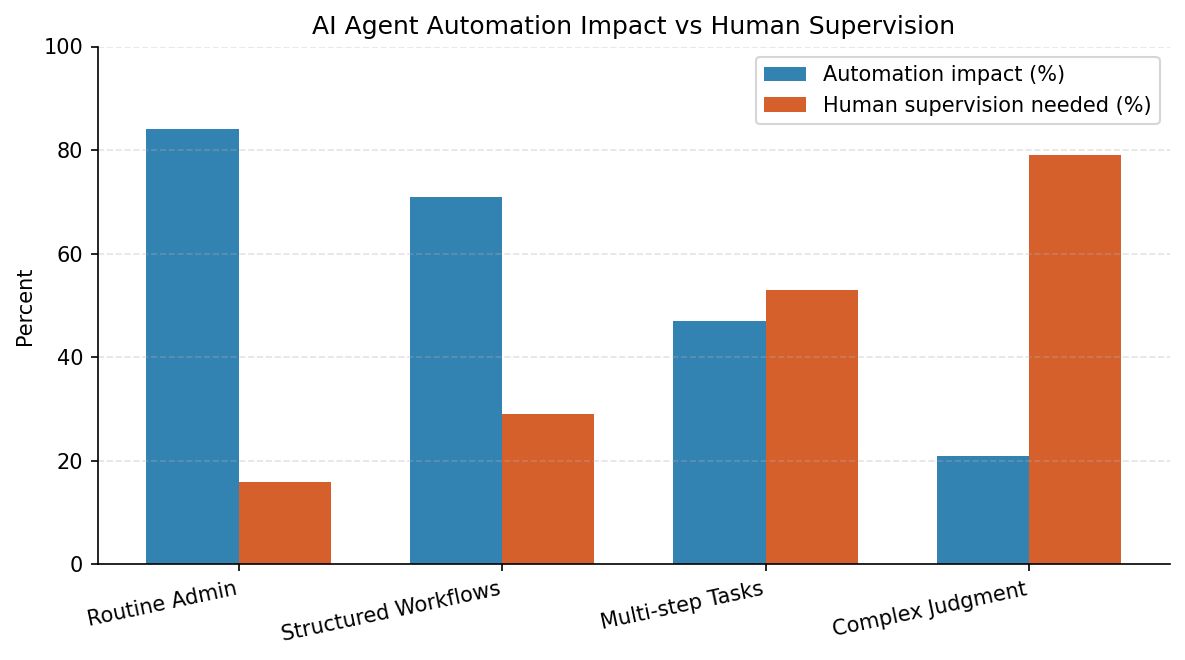
\includegraphics[width=0.92\linewidth]{automation_impact_graph.png}%
  }{%
    \begin{warningbox}{Figure unavailable}
      The automation impact chart is not available in the build output.
    \end{warningbox}
  }
  \caption{Python-generated graph: automation impact vs human supervision by task type.}
  \label{fig:automation-impact-graph}
\end{figure}

Routine administrative work shows the highest automation impact in this model, while complex
judgment tasks retain the highest supervision requirement \cite{recomaijobroles}. That
pattern supports a tiered adoption strategy: automate structured spines first, keep humans
on exception handling and approval gates \cite{arxiv2506workagents}.

\begin{insightbox}{Graph vs diagram}
The workflow diagram in Chapter~2 explains \textbf{how} real work moves through agentic
automation. This chart estimates \textbf{where} automation pressure and human supervision
concentrate in practice.
\end{insightbox}

% Professional comparison table (booktabs + tabularx).

\section{Capability Comparison}
\label{sec:capability-table}

\begin{table}[htbp]
  \centering
  \caption{Chatbot vs AI Agent vs Agentic Workflow (from live research synthesis).}
  \label{tab:capability-comparison}
  \small
  \begin{tabularx}{\linewidth}{@{}lXXX@{}}
    \toprule
    \textbf{Dimension} & \textbf{Chatbot} & \textbf{AI Agent} & \textbf{Agentic Workflow} \\
    \midrule
    Task scope & Single-turn replies & Multi-step tasks with tools &
      Orchestrated crew \emph{Process} \\
    Tool use & Limited plugins & Live search, APIs, files &
      Chained agent \emph{Tasks} with context \\
    Human oversight & Light review & \emph{Human-in-the-loop} for edge cases &
      Supervision gates per stage \\
    Risk profile & Low automation risk & Medium: bounded autonomy &
      Higher: end-to-end automation \\
  \bottomrule
  \end{tabularx}
\end{table}

\begin{insightbox}{Research alignment}
Industry commentary suggests agents reshape workflows rather than replace entire jobs
\cite{mediumworkflowagents,recomaijobroles}. Structured tasks show higher automation
potential than complex judgment work \cite{redditcomplextasks}.
\end{insightbox}

% Fancy/highlighted formula using Phase 7 formulabox macro.

\section{Automation Value Model}
\label{sec:automation-formula}

\begin{formulabox}{Automation Value (highlighted formula)}
\[
  V_{\mathrm{auto}} = T_{\mathrm{saved}} - C_{\mathrm{run}} - R_{\mathrm{risk}}
\]
\textbf{Where:}
\begin{itemize}
  \item $T_{\mathrm{saved}}$ --- time saved by automating repeatable \emph{Tasks}
  \item $C_{\mathrm{run}}$ --- compute, API, and orchestration cost per \emph{Process}
  \item $R_{\mathrm{risk}}$ --- risk cost from errors without \emph{Human-in-the-loop}
\end{itemize}
\end{formulabox}

A complementary productivity ratio used in workforce audits:

\begin{formulabox}{Human Effort Reduction}
\[
  \eta_{\mathrm{reduce}} = \frac{N_{\mathrm{automated}}}{N_{\mathrm{total}}}
  \qquad\text{with}\qquad
  0 \leq \eta_{\mathrm{reduce}} \leq 1
\]
\end{formulabox}

\begin{warningbox}{Supervision reminder}
When $\eta_{\mathrm{reduce}}$ rises, required human supervision should be re-evaluated.
Academic frameworks for delegating work to agents emphasize auditing automation boundaries
\cite{arxiv2506workagents}.
\end{warningbox}

\subsection{Using the models in practice}

Estimate $T_{\mathrm{saved}}$ from timed workflows before automation, not from vendor demos.
Record baseline minutes per research brief, draft cycle, and review pass; after deployment,
compare distributions rather than single runs \cite{recomaijobroles}. Estimate
$C_{\mathrm{run}}$ from token logs, search costs, and human review time
\cite{mediumworkflowagents}. Estimate $R_{\mathrm{risk}}$ from incident classes---bad
citations, leaked secrets, compliance exceptions---and cap $\eta_{\mathrm{reduce}}$ until
measurement improves \cite{redditcomplextasks}. A program is healthy when $V_{\mathrm{auto}}$
stays positive \emph{after} supervision and audit work is included.


% --- Chapter 4: bilingual terminology ---
\chapter{Bilingual Terminology for AI Agent Workflows}
% Chapter 4 — bilingual terminology for AI-agent workflows (Hebrew--English BiDi).

\begin{chapterintrobox}
AI-agent workflows are often designed in English, while local teams may document decisions,
approvals, and operational policy in Hebrew. This chapter defines shared terminology for
automation, supervision, and real work across both languages \cite{mediumworkflowagents}.
\end{chapterintrobox}

\section{Why Bilingual Terminology Matters}
\label{sec:bidi-why}

English dominates vendor documentation, model APIs, and agent-framework vocabulary. Yet
organizations that automate real work must explain credentials, review gates, and escalation
rules to Hebrew-speaking operators and managers. Without aligned terms, teams misread what
an \emph{Agent}, \emph{Task}, or \emph{Process} actually authorizes in production
\cite{arxiv2506workagents}.

Live workforce research asks which occupational tasks workers are willing to delegate to
agents versus keep under direct human control \cite{arxiv2506workagents}. Bilingual
terminology is therefore not cosmetic---it is how mixed-language teams agree on boundaries
before automation scales \cite{recomaijobroles}.

\section{Core English--Hebrew Terminology}
\label{sec:bidi-glossary}

Each definition below lists the English term, Hebrew equivalent, and Meaning in workflow.
Definition rows avoid tabular BiDi conflicts while keeping bilingual pairs readable.

\vspace{0.35em}
\begin{itemize}
  \item \textbf{Agent} --- \texthebrew{סוכן} --- Executes a bounded task using tools.
  \item \textbf{Task} --- \texthebrew{משימה} --- A unit of work delegated to an agent.
  \item \textbf{Crew} --- \texthebrew{צוות} --- A coordinated group of agents or roles.
  \item \textbf{Process} --- \texthebrew{תהליך} --- Ordered workflow from input to output.
  \item \textbf{API Key} --- \texthebrew{מפתח גישה} ---
    Credential used to access external services.
  \item \textbf{Human-in-the-loop} --- \texthebrew{בקרה אנושית} ---
    Human review before high-risk output.
\end{itemize}

\section{Controlled Mixed-Language Communication}
\label{sec:bidi-mixed}

\begin{insightbox}{Mixed-language example}
\textbf{Mixed-language example.} In an Israeli engineering team, a design review might use
English terms such as Agent, Task, API Key, and Human-in-the-loop, while the operational
policy is explained in Hebrew.
\end{insightbox}

\noindent
The English labels above are standard in agent platforms. The operational policy itself can
be stated in Hebrew without embedding those Latin tokens inside Hebrew sentences.

\vspace{0.35em}
\begin{hebrew}
\begin{flushright}
בדיון פנימי, הצוות מפרט את מדיניות הפעולה בעברית.
\end{flushright}
\end{hebrew}

Practitioner forums note that complex delegation still fails when boundaries are vague
\cite{redditcomplextasks}. Workflow commentary stresses agents as connectors between tools
and teams---not silent replacements for accountability \cite{mediumworkflowagents}.

\label{sec:bidi-hebrew-summary}

\begin{tcolorbox}[colback=boxBg,colframe=boxFrame,title={\texthebrew{סיכום בעברית}},sharp corners]
\begin{hebrew}
\begin{flushright}
סוכני בינה מלאכותית יכולים לבצע משימות מוגדרות כחלק מתהליך עבודה מתוזמר.\\[0.45em]
במערכת כזו, המשימה מפורקת לשלבים קטנים וברורים.\\[0.45em]
הסוכן משתמש בכלים כדי לאסוף מידע, ליצור טיוטה או לבצע פעולה.\\[0.45em]
כאשר המשימה רגישה, מסוכנת או לא ברורה, נדרשת בקרה אנושית.\\[0.45em]
המטרה אינה להחליף בני אדם לגמרי, אלא להעביר משימות מובנות לאוטומציה תוך שמירה על אחריות, פיקוח ואיכות.\\[0.45em]
לכן חשוב להגדיר מראש מתי הסוכן פועל לבד ומתי האדם חייב לאשר את התוצאה.
\end{flushright}
\end{hebrew}
\end{tcolorbox}

\section{Operational Guidance for Mixed-Language Teams}
\label{sec:bidi-practical}

When Hebrew-English teams deploy agents into real work, three practices keep automation safe:
\begin{itemize}
  \item Publish the terminology definitions in design reviews so every role shares the same
    workflow vocabulary.
  \item Store credentials and API access rules in a single authoritative runbook language,
    with Hebrew summaries where operators require them.
  \item Mark customer-facing and compliance-sensitive steps as human-in-the-loop regardless
    of language \cite{redditcomplextasks,recomaijobroles}.
\end{itemize}

\begin{warningbox}{Accountability before scale}
Automation can accelerate structured tasks in any language context, but approval language
must be explicit before agents act on consequential work \cite{arxiv2506workagents}.
\end{warningbox}


% --- Chapter 5: adoption, risks, and limits ---
\chapter{Agents, Work, and Automation}
% Chapter 5 — adoption, risks, supervision, and future-of-work themes.

\begin{chapterintrobox}
This chapter synthesizes live internet research on how AI agents change real work,
workflow automation, and organizational adoption across industries entering the agent era.
\end{chapterintrobox}

\section{What Makes AI Agents Different from Chatbots}
\label{sec:agents-vs-chatbots}

Chatbots answer prompts in a single conversational turn. AI agents pursue goals across
multiple steps: they search, call tools, write drafts, and pass context to downstream
tasks. Live commentary frames this shift as workflow orchestration rather than simple
dialogue \cite{mediumworkflowagents}.

\begin{insightbox}{Key distinction}
A chatbot optimizes for fluent replies. An agent optimizes for \emph{task completion}
inside a bounded process with tools, memory, and supervision gates.
\end{insightbox}

Agents connect signals across systems---email, tickets, documents, APIs---and reduce
handoffs that slow teams. Production teams therefore separate research, drafting, and
quality review instead of relying on one monolithic prompt \cite{mediumworkflowagents}.

Administrative automation reports show agents absorbing routine data entry and document
extraction first---high-volume, structured work \cite{recomaijobroles}. Chatbots rarely
own end-to-end outcomes in those settings because they lack persistent tool access and
review checkpoints.

\subsection{Capability boundaries}
Community practitioners note that agents excel within well-defined boundaries but struggle
when judgment, ambiguity, or cross-domain reasoning dominate
\cite{redditcomplextasks}. The gap between ``automate a workflow step'' and ``replace a
profession'' remains wide in live discussions.

\section{Tool Use and Workflow Automation}
\label{sec:tool-use}

Modern agent stacks treat tools as first-class interfaces: search services, document
repositories, ticketing systems, and enterprise API connectors. Each tool invocation is a
\emph{Task} with an auditable input and output, which supports traceability in regulated
environments.

\begin{insightbox}{Workflow pattern}
Typical pattern: \textbf{search} $\rightarrow$ \textbf{synthesize} $\rightarrow$
\textbf{draft} $\rightarrow$ \textbf{review} $\rightarrow$ \textbf{publish}. Each stage
can fail independently and be retried without corrupting upstream evidence.
\end{insightbox}

Workflow automation value rises when agents observe events, prioritize work, and route
tasks between humans and software \cite{mediumworkflowagents}. Tool use is therefore not a
feature list---it is the mechanism that turns language models into operators.

Academic auditing frameworks ask which occupational tasks workers would delegate to
agents versus keep under human control \cite{arxiv2506workagents}. Tool-enabled agents make
those trade-offs explicit: every automated step should map to a named capability and a
supervision policy.

\subsection{Orchestration in practice}
Sequential orchestration runs specialized agents with shared context. That design mirrors
how organizations already separate research, drafting, and quality review---but at higher
speed and with live source retrieval. Chapter~2 illustrates how structured tasks flow through
agent automation; Chapter~3 quantifies where automation impact is highest across supervision
models.

\section{Human-in-the-Loop Supervision}
\label{sec:human-in-loop}

\emph{Human-in-the-loop} review is not optional for high-impact automation. Operators
approve agent plans, validate citations, and intercept errors before publication or
customer-facing actions. Research on occupational delegation stresses auditing which tasks
workers trust agents to perform \cite{arxiv2506workagents}.

\begin{warningbox}{Supervision principle}
Increase automation scope only when monitoring cost stays lower than the value of
delegated work. If review queues grow faster than throughput, the agent design is likely
too autonomous for the risk profile.
\end{warningbox}

Supervision tiers can be documented as:
\begin{itemize}
  \item \textbf{Observe:} human watches logs and metrics only.
  \item \textbf{Approve:} human confirms before external side effects.
  \item \textbf{Collaborate:} human and agent iterate on the same task.
  \item \textbf{Escalate:} agent hands off when confidence or policy thresholds fail.
\end{itemize}

Reddit practitioners highlight that multi-step agents need clear stop conditions when
tasks exceed training or tool boundaries \cite{redditcomplextasks}. Production systems
should encode those stops as policy, not hope the model improvises safely.

\section{Risks, Guardrails, and Failure Modes}
\label{sec:risks-guardrails}

Agent failures differ from chatbot failures. A wrong answer becomes a wrong action: bad
citations, leaked secrets, duplicated customer emails, or corrupted documents. Guardrails
therefore span data access, tool permissions, and output validation---not just prompt
engineering.

\begin{warningbox}{Common failure modes}
\begin{itemize}
  \item Hallucinated sources that look plausible in draft text.
  \item Over-automation of judgment-heavy decisions.
  \item Credential exposure through logs or prompts.
  \item Runaway tool loops without budget or time limits.
\end{itemize}
\end{warningbox}

Mitigations align with the automation value model in Chapter~3: track runtime cost
$C_{\mathrm{run}}$, estimate risk cost $R_{\mathrm{risk}}$, and require human gates when
expected loss exceeds savings. Administrative automation case studies show large gains in
routine roles but also role redesign rather than silent elimination
\cite{recomaijobroles}.

\section{Business Adoption and the Future of Work}
\label{sec:business-adoption}

Enterprises adopt agents where friction is measurable: ticket triage, research briefs,
compliance checklists, and document pipelines. The near-term story is less ``fewer jobs''
and more ``fewer manual handoffs''---agents sit between teams and systems
\cite{mediumworkflowagents}.

\begin{insightbox}{Adoption lens}
Measure adoption by \textbf{workflow latency} and \textbf{error rework}, not only headcount.
Agents that shorten review cycles while improving citation quality justify continued
investment even when full replacement is unrealistic.
\end{insightbox}

Workforce auditing research proposes structured evaluation of which tasks employees want
automated versus augmented \cite{arxiv2506workagents}. That employee-centered framing
reduces backlash and produces guardrails grounded in real job constraints.

Industry reporting on administrative roles shows concrete task displacement patterns---
data entry, scheduling support, extraction---while strategic decisions remain human-led
\cite{recomaijobroles}. Future-of-work narratives should separate \emph{task automation}
from \emph{role erasure}.

\subsection{Organizational readiness}
Readiness checklist for agent deployment:
\begin{itemize}
  \item Live source policy: which APIs and search tools are approved?
  \item Secret management: keys outside prompts and version control.
  \item Review ownership: who signs drafts before external release?
  \item Evidence retention: store search results and agent logs for audit.
  \item Rollback plan: how to revert automated changes quickly.
\end{itemize}

\section{Limitations of Full Automation}
\label{sec:limitations}

Full automation---agents operating without meaningful human oversight---is rarely credible
for complex, high-stakes work. Practitioners report agents handling multi-step routines but
failing when goals are underspecified or tools are incomplete
\cite{redditcomplextasks}.

\begin{warningbox}{Realistic expectation}
Agents are force multipliers for structured work, not universal substitutes for expertise.
The central theme---agents that replace \emph{real work}---must be read as selective
automation of tasks, not total workforce replacement.
\end{warningbox}

Limitations cluster into four areas:
\begin{enumerate}
  \item \textbf{Context limits:} agents lose thread across long, branching projects.
  \item \textbf{Judgment limits:} ethical, legal, and brand decisions need human owners.
  \item \textbf{Tool limits:} agents cannot act where APIs or data are unavailable.
  \item \textbf{Verification limits:} citations and numbers require independent checks
    \cite{arxiv2506workagents}.
\end{enumerate}

Sustainable programs treat agents as teammates in a supervised \emph{Process}: automate
the repetitive spine of work, keep humans on the margins where variance and accountability
concentrate. That posture matches both academic auditing models and practitioner caution in
live forums \cite{redditcomplextasks,mediumworkflowagents}.

\section{Evidence Retention and Audit Trails}
\label{sec:audit-trails}

Automated research and drafting are only defensible when organizations retain evidence.
Each agent stage should persist inputs and outputs: source records, intermediate drafts,
approval notes, and published deliverables. That mirrors how compliance teams reconstruct
decisions after incidents \cite{arxiv2506workagents}.

\begin{insightbox}{Audit practice}
Store \textbf{who} triggered a run, \textbf{which tools} were called, \textbf{what sources}
were retrieved, and \textbf{who approved} external publication. Agents without audit trails
are difficult to defend in enterprise settings.
\end{insightbox}

Audit trails also reduce citation hallucination risk. When reviewers can compare draft
claims to stored source snippets, false references surface before publication.
Administrative automation programs report the same pattern: automation succeeds when
document provenance is explicit \cite{recomaijobroles}.

\subsection{Minimum evidence package}
\begin{itemize}
  \item Timestamped source records with URLs and titles.
  \item Intermediate drafts with role labels (research, draft, approval).
  \item Review outcomes covering accuracy, clarity, and policy alignment.
  \item Published outputs with version identifiers.
  \item Runtime and cost summaries for budget governance.
\end{itemize}

\section{Measuring Agent Program Success}
\label{sec:metrics}

Organizations should score agent programs with operational metrics, not hype metrics.
Vanity metrics---``number of prompts'' or ``model upgrades''---do not prove work was replaced
safely.

\begin{table}[htbp]
  \centering
  \caption{Sample metrics for agent automation programs.}
  \label{tab:agent-metrics}
  \small
  \begin{tabularx}{\linewidth}{@{}lXX@{}}
    \toprule
    \textbf{Metric} & \textbf{What it measures} & \textbf{Why it matters} \\
    \midrule
    Cycle time & Hours from research to approved draft & Workflow speed \\
    Rework rate & Share of drafts sent back for revision & Quality and supervision \\
    Source coverage & Citations tied to live URLs & Research integrity \\
    Escalation rate & Tasks routed to humans & Boundary respect \\
    Cost per outcome & API spend per published artifact & Financial guardrail \\
    \bottomrule
  \end{tabularx}
\end{table}

Academic workforce auditing suggests measuring \emph{which tasks workers want delegated}
rather than assuming universal enthusiasm for automation
\cite{arxiv2506workagents}. Pair that qualitative signal with the quantitative table above.

\begin{warningbox}{Metric trap}
Do not reward agents for volume alone. Publishing more drafts with weak citations increases
rework and reputational risk faster than it saves labor \cite{redditcomplextasks}.
\end{warningbox}

\subsection{Quarterly review questions}
\begin{enumerate}
  \item Which workflows gained measurable latency reduction?
  \item Where did human review time increase instead of decrease?
  \item Did live source diversity improve or narrow?
  \item Which tool permissions should be tightened?
  \item Are high-risk tasks still behind human approval gates?
\end{enumerate}

Answering these questions keeps agent programs aligned with the book's central theme:
\textbf{AI agents that replace real work}---meaning specific, evidenced tasks---rather than
unbounded promises of full workforce replacement \cite{mediumworkflowagents,recomaijobroles}.

\section{Deployment Checklist for Production Agents}
\label{sec:deployment-checklist}

Before running agents against live APIs in production, teams should verify environment,
governance, and rollback mechanics. The checklist below summarizes practices supported by
live research on workflow agents \cite{mediumworkflowagents,arxiv2506workagents}.

\begin{enumerate}
  \item \textbf{Govern credentials:} store API keys and tokens outside prompts and
    version-controlled content.
  \item \textbf{Validate tools:} confirm connectors return authoritative data before
    drafting or executing actions.
  \item \textbf{Scope rollouts:} start with one workflow; expand only after latency and
    rework metrics improve \cite{recomaijobroles}.
  \item \textbf{Validate outputs:} ensure drafts and citations match retrieved evidence.
  \item \textbf{Maintain references:} linked citations must map to a curated bibliography.
  \item \textbf{Archive artifacts:} retain source records, drafts, approvals, and audit logs.
  \item \textbf{Review high-risk text:} require human sign-off when outputs mention job
    replacement or unverified claims \cite{redditcomplextasks}.
\end{enumerate}

\begin{insightbox}{Production mindset}
Treat each agent pipeline execution as a \textbf{publishable workflow}, not a demo. The
difference is evidence: stored artifacts, linked citations, and reproducible outputs.
\end{insightbox}

Administrative automation case studies emphasize phased rollout: automate one workflow,
measure rework and latency, then expand tool permissions gradually
\cite{recomaijobroles}. Skipping phases produces brittle programs that break when models,
APIs, or policies change.

Finally, communicate limits openly. Agents that augment workflows can earn trust; agents
marketed as flawless replacements trigger resistance and hidden manual work
\cite{mediumworkflowagents,redditcomplextasks}. Honest limitation language is part of
professional design---not a weakness in the automation story.


\printbibliography[heading=bibintoc,title={References}]

\end{document}
